\section{Metric spaces}

% Offering-specific handouts may begin immediately after Example 2.2.
% Preserve the theorem numbering from the master notes.
\ifdefined\startafterexampletwotwo
  \setcounter{theorem}{2}
\else

For real functions $f:\R\to\R$, we have the notion of continuity using $\varepsilon$-$\delta$ definition: a function $f:\R\to\R$ is continuous at a point $x_0\in\R$ if for every $\varepsilon>0$ there exists $\delta>0$ such that
\[
|f(x)-f(x_0)|<\varepsilon \quad \text{whenever } |x-x_0|<\delta.
\]
We also have the notion of continuity using sequences: a function $f:\R\to\R$ is continuous at a point $x_0\in\R$ if for every sequence $(x_n)$ in $\R$ converging to $x_0$, the sequence $(f(x_n))$ converges to $f(x_0)$. 

In an attempt to generalize these notions to more general settings than $\R$, Frechet introduced the notion of metric spaces in 1906. Metric spaces provide a natural setting to generalize the notions of continuity above. Later, Hausdorff introduced the more general notion of topological spaces in 1914. We will first study metric spaces and then topological spaces.

\begin{definition}[Metric Space]
A \emph{metric space} is a pair $(X,d)$ consisting of a set $X$ and a
function $d\colon X\times X\to [0,\infty)$ called a \emph{metric} such that
\begin{enumerate}
  \item $d(x,y)=0$ if and only if $x=y$;
  \item $d(x,y)=d(y,x)$ for all $x,y\in X$ (symmetry);
  \item $d(x,z)\le d(x,y)+d(y,z)$ for all $x,y,z\in X$ (triangle inequality).
\end{enumerate}
The value $d(x,y)$ is called the \emph{distance} between points $x$ and $y$ in the metric space.

If $(X,d)$ satisfies 2 and 3 and 1' below, it is called a \emph{pseudometric space}. 

1'. $d(x,x)=0$ for all $x\in X$.
\end{definition}

\begin{example}
  \begin{enumerate}
    \item $X=\R^n$, $d_p(x,y)=\|x-y\|_p=\left(\sum_{i=1}^n |x_i-y_i|^p\right)^{1/p}$ for $1\le p<\infty$ and $d_\infty(x,y)=\|x-y\|_\infty=\max_{1\le i\le n}|x_i-y_i|$ are metrics on $\R^n$. 
    \item Let $X$ be any set and $f:X\to \R$ be any function. Then, the following defines a pseudometric on $X$:
      \[
      d(x,y) = |f(x)-f(y)|.
      \]
    \item Let $(X,d)$ be a metric space and $A\subset X$ be a nonempty subset. Then, $(A,d|_{A\times A})$ is a metric space, called a \emph{subspace} of $(X,d)$.
  \end{enumerate}
\end{example}

\fi

% Offering-specific weekly handouts may stop after Example 2.2.
\ifdefined\stopafterexampletwotwo
  \expandafter\endinput
\fi



\begin{definition}
  Let $(X,d_X)$ and $(Y,d_Y)$ be metric spaces. A function $f\colon X\to Y$ is called an isometric embedding if
  \[
  d_Y(f(x),f(x'))=d_X(x,x') \quad \text{for all } x,x'\in X.
  \]
  The function $f$ is called an isometry if it is an isometric embedding that is also surjective and we say that $(X,d_X)$ and $(Y,d_Y)$ are \emph{isometric} if there exists an isometry between them.
\end{definition}

\begin{example}[Isometric embedding]
Let $f:\R\to\R^2$ be given by $f(t)=(t,0)$. For $s,t\in\R$,
\[
\|f(s)-f(t)\|_2=\sqrt{(s-t)^2+0^2}=|s-t|.
\]
Thus $f$ preserves distances (an isometric embedding). It is not surjective, so it is not an isometry. Its image is the $x$-axis in $\R^2$.

Is the map $g(x):=(x,x)$ an isometric embedding?
\end{example}





\begin{definition}
  Let $(X,d_X)$ and $(Y,d_Y)$ be metric spaces. A function $f\colon X\to Y$ is called \emph{Lipschitz continuous} if there exists a constant $L\ge 0$ such that
  \[
  d_Y(f(x),f(x'))\le L \cdot d_X(x,x') \quad \text{for all } x,x'\in X.
  \]
\end{definition}

\begin{definition}
  Let $(X,d_X)$ and $(Y,d_Y)$ be metric spaces. A function $f\colon X\to Y$ is called \emph{continuous} at a point $x_0\in X$ if for every $\varepsilon>0$ there exists $\delta>0$ such that
  \[
  d_Y(f(x),f(x_0))<\varepsilon \quad \text{whenever } d_X(x,x_0)<\delta.
  \]
  The function $f$ is called \emph{continuous} if it is continuous at every point $x_0\in X$.
\end{definition}


\begin{proposition}
  Any Lipschitz continuous function between metric spaces is continuous. Any isometric embedding is also Lipschitz continuous.
\end{proposition}
\begin{proof}
  Let $f:X\to Y$ be Lipschitz continuous with constant $L$. Given $\varepsilon>0$, let $\delta=\varepsilon/L$. Then, for any $x\in X$ with $d_X(x,x_0)<\delta$, we have
  \[
  d_Y(f(x),f(x_0))\le L\cdot d_X(x,x_0)<L\cdot \frac{\varepsilon}{L}=\varepsilon.
  \]
  Thus, $f$ is continuous at $x_0$. Since $x_0$ is arbitrary, $f$ is continuous.

  If $f$ is an isometric embedding, then for any $x,x'\in X$, we have
  \[
  d_Y(f(x),f(x'))=d_X(x,x')\le 1\cdot d_X(x,x').
  \]
  Thus, $f$ is Lipschitz continuous with constant $L=1$.
\end{proof}



\subsection{Characterizations of continuity}

\subsubsection{A sequential characterization of continuity}

For real functions, we can define continuity using sequences. This can be generalized to metric spaces as well.

\begin{definition}
    A sequence $(x_n)_{n\in\mathbb{N}}$ in a metric space $(X,d)$ is said to converge to a point $x\in X$ if for every $\epsilon>0$, there exists $N\in\mathbb{N}$ such that $d(x_n,x)<\epsilon$ for all $n\ge N$.
\end{definition}

One can characterize continuity using sequences:
\begin{proposition}
    A function $f:X\to Y$ is continuous at a point $x_0\in X$ if and only if for every sequence $(x_n)_{n\in\mathbb{N}}$ in $X$ converging to $x_0$, the sequence $(f(x_n))_{n\in\mathbb{N}}$ converges to $f(x_0)$.
\end{proposition}
\begin{proof}
  Suppose first that $f$ is continuous at $x_0$, and let $(x_n)_{n\in\mathbb{N}}$ be a sequence converging to $x_0$. For any $\varepsilon>0$, by continuity there exists $\delta>0$ such that
  \[
  d_X(x,x_0)<\delta \quad\Longrightarrow\quad d_Y(f(x),f(x_0))<\varepsilon.
  \]
  Since $(x_n)$ converges to $x_0$, there exists an $N\in\mathbb{N}$ with $d_X(x_n,x_0)<\delta$ for all $n\ge N$. Hence, for all $n\ge N$, we have
  \[
  d_Y(f(x_n),f(x_0))<\varepsilon,
  \]
  so $(f(x_n))$ converges to $f(x_0)$.

  Conversely, suppose that for every sequence $(x_n)$ converging to $x_0$, the sequence $(f(x_n))$ converges to $f(x_0)$. Assume for contradiction that $f$ is not continuous at $x_0$. Then there exists $\varepsilon_0>0$ such that for every $\delta>0$ there exists some $x\in X$ with
  \[
  d_X(x,x_0)<\delta \qquad\text{but}\qquad d_Y(f(x),f(x_0))\ge \varepsilon_0.
  \]
  For each $n\in\mathbb{N}$, choosing $\delta=\frac{1}{n}$, there exists $x_n\in X$ with
  \[
  d_X(x_n,x_0)<\frac{1}{n} \quad\text{and}\quad d_Y(f(x_n),f(x_0))\ge \varepsilon_0.
  \]
  Then $(x_n)$ converges to $x_0$, yet $(f(x_n))$ cannot converge to $f(x_0)$ since the distance remains at least $\varepsilon_0$, which is a contradiction.
\end{proof}

\subsubsection{A open set characterization of continuity}

\begin{definition}
  Let $(X,d)$ be a metric space. For any $x\in X$ and $r>0$, the \emph{open ball} of radius $r$ centered at $x$ is defined as
  \[
  B_r(x) = \{y\in X:d(x,y)<r\}.
  \]
\end{definition}

\begin{example}[Shapes of balls for different metrics on \(\R^2\)]
For \(r>0\) the open unit balls (centered at the origin) for the standard metrics on \(\R^2\) have the following shapes:
\[
\begin{aligned}
B_r^{(2)}(0) &= \{x\in\R^2 : \|x\|_2 < r\}      &&\text{(Euclidean) — disk},\\
B_r^{(1)}(0) &= \{x\in\R^2 : |x_1|+|x_2| < r\}  &&\text{(Taxicab / \(\ell^1\)) — diamond},\\
B_r^{(\infty)}(0) &= \{x\in\R^2 : \max(|x_1|,|x_2|) < r\} &&\text{(Maximum / \(\ell^\infty\)) — square}.
\end{aligned}
\]
Below we draw the case \(r=1\).
\end{example}

\begin{figure}[h]
  \centering
  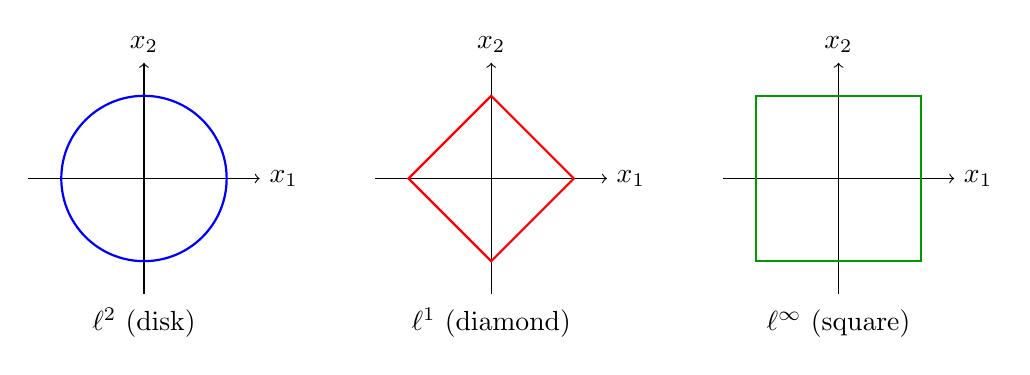
\begin{tikzpicture}[scale=1.05]
    % Euclidean ball
    \begin{scope}
      \draw[->] (-1.4,0)--(1.4,0) node[right]{$x_1$};
      \draw[->] (0,-1.4)--(0,1.4) node[above]{$x_2$};
      \draw[thick,blue] (0,0) circle (1);
      \node at (0,-1.75) {\(\ell^2\) (disk)};
    \end{scope}
    % Taxicab ball
    \begin{scope}[xshift=4.2cm]
      \draw[->] (-1.4,0)--(1.4,0) node[right]{$x_1$};
      \draw[->] (0,-1.4)--(0,1.4) node[above]{$x_2$};
      \draw[thick,red] (0,1)--(1,0)--(0,-1)--(-1,0)--cycle;
      \node at (0,-1.75) {\(\ell^1\) (diamond)};
    \end{scope}
    % Infinity ball
    \begin{scope}[xshift=8.4cm]
      \draw[->] (-1.4,0)--(1.4,0) node[right]{$x_1$};
      \draw[->] (0,-1.4)--(0,1.4) node[above]{$x_2$};
      \draw[thick,green!60!black] (-1,-1) rectangle (1,1);
      \node at (0,-1.75) {\(\ell^\infty\) (square)};
    \end{scope}
  \end{tikzpicture}
  \caption{Unit balls \(B_1(0)\) in \(\R^2\) for \(\ell^2,\ \ell^1,\ \ell^\infty\) metrics.}
\end{figure}

Then, we can rewrite the definition of continuity using open balls.

\begin{proposition}
  A function $f:X\to Y$ between metric spaces $(X,d_X)$ and $(Y,d_Y)$ is continuous at a point $x_0\in X$ if and only if for every $r>0$, there exists $\delta>0$ such that
  \[
  f(B_\delta(x_0))\subseteq B_r(f(x_0)).
  \]
\end{proposition}

The definition of open balls of course depends on the metric. Suppose you want to generalize everything so far to the setting when you don't have metric. Then, let's try to define some language where the notion of metric will be hidden. 

\begin{definition}
      A subset $U\subseteq X$ is called \emph{open} if for every point $x\in U$ there exists a radius $r>0$ such that the open ball $B_r(x)$ is contained in $U$.
\end{definition}

\begin{proposition}
  Any open ball $B_r(x)$ is open.
\end{proposition}
\begin{proof}
  Let's prove the last item. Let $x\in B_r(x_0)$ for some $r>0$. Pick $r':=r-d_X(x,x_0)$. Then, $B_{r'}(x)\subseteq B_r(x_0)$.
\end{proof}

\begin{corollary}
  Let $(X,d)$ be a metric space and $U\subseteq X$ be a subset. Then, $U$ is open iff $U$ is a union of open balls.
\end{corollary}

\begin{proof}
  Assume that $U$ is open. Then, for every $x\in U$ there exists $r_x>0$ so that $B_{r_x}(x)\subseteq U$. Thus, we can write
  \[
  U = \bigcup_{x\in U} B_{r_x}(x).
  \]

  Conversely, if $U=\bigcup_{i\in I}B_{r_i}(x_i)$ is a union of open balls, then for every $x\in U$, we have that $x\in B_{r_i}(x_i)$ for some $i\in I$. This means that there exists a radius $r>0$ such that $B_r(x)\subseteq B_{r_i}(x_i)\subseteq U$. Thus, $U$ is open.
\end{proof}

% \begin{proposition}
%   Let $(X,d)$ be a metric space.
%   \begin{enumerate}
%     \item The empty set is open
%     \item The whole space $X$ is open.
%     \item Any union of open sets is open.
%     \item The intersection of two open sets is open. Hence, the intersection of any finite number of open sets is open.
%   \end{enumerate}
% \end{proposition}

Now we can revisit the definition of continuous functions.

\begin{theorem}
  Let $f:X\to Y$ be a function between metric spaces $(X,d_X)$ and $(Y,d_Y)$. Then $f$ is continuous at a point $x_0\in X$ if and only if for every open set $V\subseteq Y$ containing $f(x_0)$, there exists an open set $U\subseteq X$ containing $x_0$ such that $f(U)\subseteq V$. 
\end{theorem}
\begin{proof}
  Suppose that $f$ is continuous at $x_0$. Let $V\subseteq Y$ be an open set containing $f(x_0)$. By openness, there exists $r>0$ such that $B_r(f(x_0))\subseteq V$. By continuity, there exists $\delta>0$ such that $f(B_\delta(x_0))\subseteq B_r(f(x_0))\subseteq V$. Thus, we can take $U=B_\delta(x_0)$.

  Conversely, suppose that for every open set $V\subseteq Y$ containing $f(x_0)$, there exists an open set $U\subseteq X$ containing $x_0$ such that $f(U)\subseteq V$. Given $\varepsilon>0$, let $V=B_\varepsilon(f(x_0))$. By assumption, there exists an open set $U\subseteq X$ containing $x_0$ such that $f(U)\subseteq V$. Since $U$ is open and contains $x_0$, there exists $\delta>0$ such that $B_\delta(x_0)\subseteq U$. Thus,
  \[
  f(B_\delta(x_0))\subseteq f(U)\subseteq V = B_\varepsilon(f(x_0)).
  \]
  This shows that $f$ is continuous at $x_0$. 
\end{proof}

Finally, we will be able to establish the following characterization from the theorem above. We will not give a proof here as we will give a proof in a more general setting (topological spaces) later.

\begin{theorem}
  $f$ is continuous if and only if for every open set $V\subseteq Y$, the preimage $f^{-1}(V)$ is open in $X$.
\end{theorem}

The above theorem reads "preimage of open is open".


\subsubsection{A closed set characterization of continuity}
However, I never find this characterization natural to understand. We can think of the continuity as not ripping apart the space at any given point. More precisely, if a point is ``in touch'' with some region in the domain, it should remain in touch with the corresponding region in the codomain.

\begin{figure}[h!]
\centering
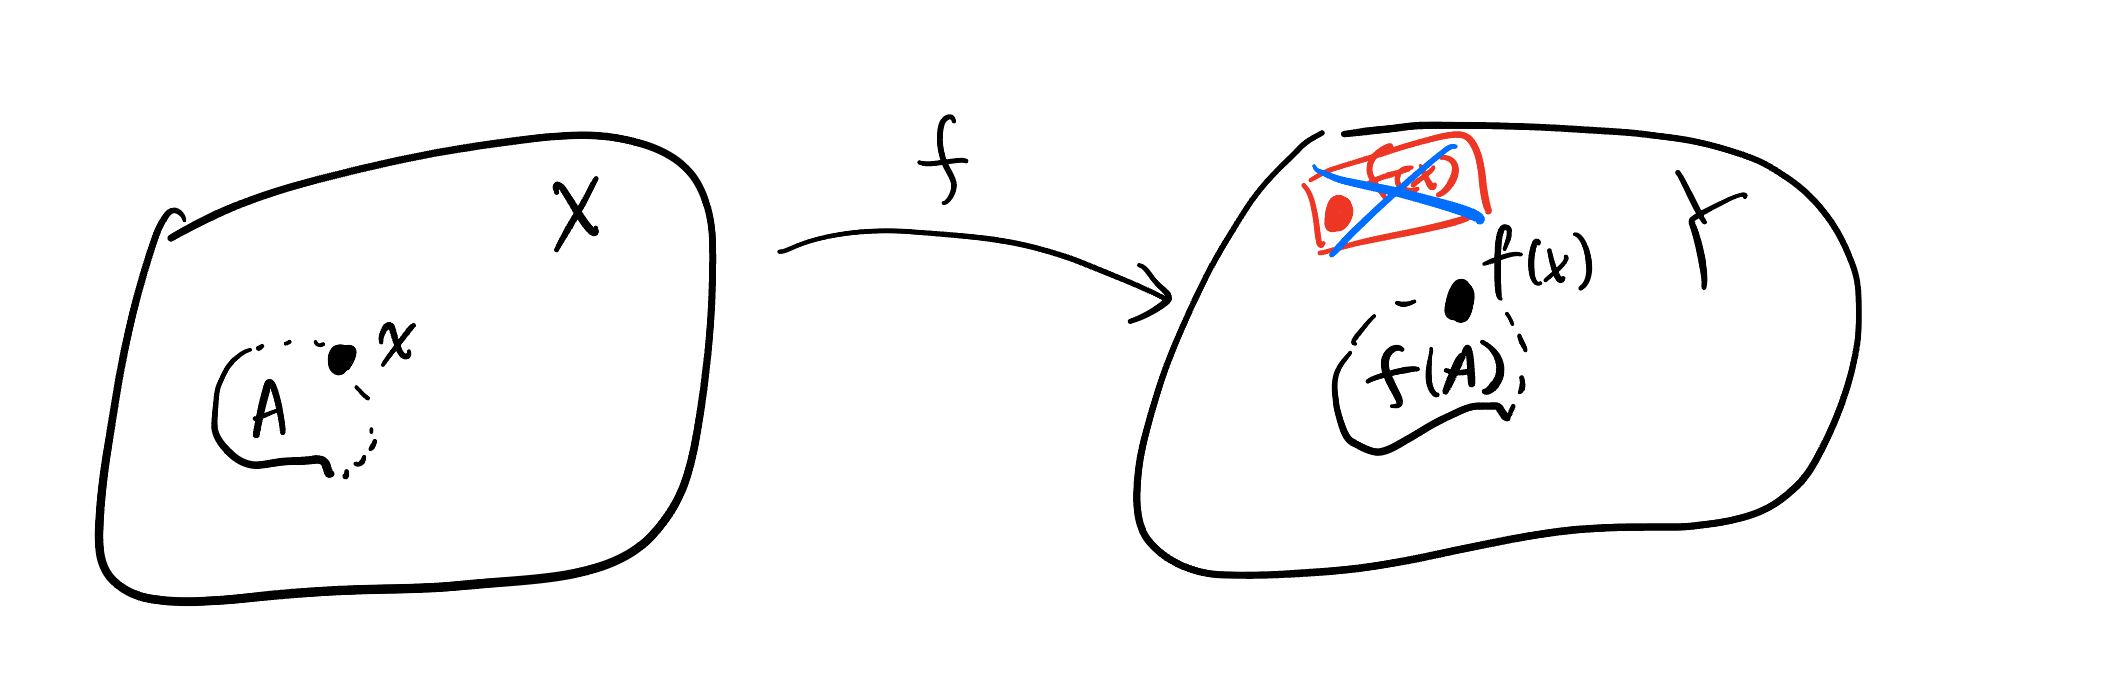
\includegraphics[width=0.8\textwidth]{figures/close-continuity.png}
\label{fig:close-continuity}
\end{figure}


\begin{definition}
  A subset $A\subseteq X$ is called \emph{closed} if its complement $X\setminus A$ is open. 
\end{definition}
% \begin{proposition}
%   Let $(X,d)$ be a metric space.
%   \begin{enumerate}
%     \item The empty set is closed.
%     \item The whole space $X$ is closed.
%     \item Any intersection of closed sets is closed.
%     \item The union of two closed sets is closed. Hence, the union of any finite number of closed sets is closed.
%   \end{enumerate}
% \end{proposition}


\begin{definition}
  For any set $A\subseteq X$, the \emph{closure} of $A$, denoted $\overline{A}$, is the smallest closed set containing $A$. Equivalently, it is the intersection of all closed sets containing $A$.
\end{definition}

\begin{theorem}\label{thm:image-closure}
  Let $f:X\to Y$ be a function between metric spaces $(X,d_X)$ and $(Y,d_Y)$. Then $f$ is continuous if and only if $f(\overline{A})\subseteq\overline{f(A)}$
\end{theorem}

The theorem above reads "image of closure is contained in closure of image", or more intuitively, "points that are in touch with a set remains in touch after the map".


Now we prove the theorem.

\begin{lemma}
  Let $A\subseteq X$ be a set. Then,
  \[\overline{A} = \{x\in X : \text{there exists a sequence }(x_n)_{n\in\mathbb{N}}\text{ in }A\text{ converging to }x\}.\]
\end{lemma}
\begin{proof}
  Let $x\in\overline{A}$. Consider any $r>0$. If $B_r(x)\cap A=\emptyset$, then the complement $X\backslash B_r(x)\supset A$. But this contradicts the fact that $x\in\overline{A}$. Now let $r_n:=1/n$. Then, pick $x_n\in B_{r_n}(x)\cap A$. Then, $(x_n)$ is a sequence in $A$ converging to $x$.

  Conversely, let $x\in X$ be such that there exists a sequence $(x_n)_{n\in\mathbb{N}}$ in $A$ converging to $x$. Consider a closed set $C\supset A$. If $x\notin C$, then there exists $r>0$ such that $B_r(x)\cap C=\emptyset$ (why?). This implies that $B_r(x)\cap A=\emptyset$ which contradicts the fact that $(x_n)$ converges to $x$. Thus, $x\in C$. Since $C\supset A$ is arbitrary, we have $x\in\overline{A}$. 
\end{proof}

Now, we prove \Cref{thm:image-closure}.
\begin{proof}[Proof of \Cref{thm:image-closure}]
  Suppose that $f$ is continuous. Let $x\in\overline{A}$. By the lemma, there exists a sequence $(x_n)$ in $A$ converging to $x$. By continuity, $(f(x_n))$ converges to $f(x)$. Since each $f(x_n)\in f(A)$, by the lemma again, we have $f(x)\in\overline{f(A)}$. Thus, $f(\overline{A})\subseteq\overline{f(A)}$.

  Conversely, suppose that $f(\overline{A})\subseteq\overline{f(A)}$ for every set $A\subseteq X$. Let $x_0\in X$ and let $(x_n)$ be a sequence converging to $x_0$. Assume on the contrary that $(f(x_n))$ does not converge to $f(x_0)$. Then, there exists $\varepsilon>0$ such that there is a subsequence $(f(x_{k_n}))$ such that $d_Y(f(x_{k_n}),f(x_0))\ge \varepsilon$ for all $n\in\mathbb{N}$.

  Now we let $A=\{x_{k_n}:n\in\mathbb{N}\}$. Then, $x_0\in\overline{A}$. Thus, $f(x_0)\in f(\overline{A})\subseteq \overline{f(A)}$. By the lemma, there exists a sequence $(y_n)$ in $f(A)$ converging to $f(x_0)$. But this is not possible due to the $\epsilon$ constraint. Therefore, we conclude that $(f(x_n))$ must converge to $f(x_0)$.
\end{proof}

We now see that many intuitive properties of continuous real functions can be generalized nicely to metric spaces. We will see that the open and closed language still works well in the more general setting of topological spaces, while the sequential language does not. In Willard's book, a whole chapter is devoted to the study of sequences in topological spaces.

\subsection{Ultrametric}
There is a special class of metric spaces called ultrametric spaces, which satisfy a stronger version of the triangle inequality. Ultrametric spaces have some interesting properties that are not shared by general metric spaces.

\begin{definition}[Ultrametric space]
A metric space $(X,d)$ is an \emph{ultrametric space} if $d$ satisfies the
\emph{strong triangle inequality}
\[
d(x,z)\le \max\{d(x,y),d(y,z)\}\qquad \text{for all }x,y,z\in X.
\]
We would usually use $u$ instead of $d$ to denote an ultrametric.
\end{definition}

\begin{proposition}
  Let $(X,u)$ be an ultrametric space. Then,
\begin{enumerate}
  \item If $r>0$ and $x,y\in X$ with $u(x,y)<r$, then $B_r(x)=B_r(y)$.
  \item Any two open balls are either disjoint or one contains the other.
  \item Every triangle is isosceles, i.e., if $x,y,z\in X$, then at least two of the distances $u(x,y)$, $u(y,z)$, and $u(z,x)$ are equal, and the third is less than or equal to the common value.
\end{enumerate}
\end{proposition}

\begin{example}
  Recall the definition of the Cantor set $C\subseteq [0,1]$: it is constructed by repeatedly removing the open middle third from each interval. More precisely, set $C_0 = [0,1]$, and for each $k\ge 1$, let $C_k$ be the union of $2^k$ closed intervals obtained by removing the open middle third from each interval in $C_{k-1}$. The Cantor set is defined as
  \[
  C = \bigcap_{k=0}^\infty C_k.
  \]
  Equivalently, $C$ consists of all numbers in $[0,1]$ whose base-3 expansion contains only the digits $0$ and $2$.
  We endow the Cantor set $C\subseteq [0,1]$ with the ultrametric as follows:
  \[
  d_C(x,y) =
  \begin{cases}
  0 & \text{if } x=y,\\[1ex]
  3^{-n} & \text{if } x\neq y \text{ and } n = \min\{ k \ge 0 : \text{$x$ and $y$ lie in different segments in } C_k \}.
  \end{cases}
  \]
\end{example}

It is perhaps difficult for you to understand what happens in the example above. It turns out that one can always create a nice visualization of ultrametric spaces using trees. We will use this to help us understand ultrametric spaces better. Although the following definition is for finite sets, it can be generalized to infinite sets as well.

\newpage

\begin{definition}
  \textbf{Dendrogram (finite case).}
  Let $X$ be finite. A dendrogram on $X$ is an order preserving map $\theta:[0,\infty)\to Part(X)$ on $X$ such that:
  \begin{enumerate}
    \item $\theta(0)$ is the discrete partition of $X$;
    \item there exists $T>0$ such that $\theta(T)$ is the trivial partition;
    \item for any $t\geq 0$, there exists $\epsilon>0$ such that $\theta(t)=\theta(t+\epsilon)$.
  \end{enumerate}
\end{definition}
\begin{example}
  Consider $X=\{a,b,c\}$. Define $\theta:[0,\infty)\to Part(X)$ by
  \[
  \theta(t) =
  \begin{cases}
    \{\{a\},\{b\},\{c\}\} & \text{if } 0\le t<1 \\
    \{\{a,b\},\{c\}\} & \text{if } 1\le t<2 \\
    \{\{a,b,c\}\} & \text{if } t\ge 2
  \end{cases}
  \]
  Notice that the strict inequalities cannot be replaced with non-strict inequalities, as this would violate the last condition.
\end{example}



\begin{theorem}[Finite dendrograms and ultrametrics are equivalent]
Let $X$ be a finite set. Let $\mathcal{D}(X)$ be the set of dendrograms on $X$ and $\mathcal{U}(X)$ be the set of ultrametrics on $X$. There are two maps between $\mathcal{D}(X)$ and $\mathcal{U}(X)$ as follows:
\begin{enumerate}
  \item (From dendrogram to ultrametric) Given a dendrogram $\theta$ on $X$, define
  \[
    u(x,y):=\inf\{t\ge 0:\ x, y \text{ belong to the same block in }\theta(t)\}\quad (x,y\in X).
  \]
  Then $u$ is an ultrametric on $X$.
  \item (From ultrametric to dendrogram) Given an ultrametric $u$ on $X$ set, we define an equivalence relation $\sim_t$ for $t\ge 0$,
  \[
    x\sim_t y \;\Longleftrightarrow\; u(x,y)\le t.
  \]
  Then we define $\theta$ by $\theta(t):=\{[x]_t:x\in X\}$ where $[x]_t$ is the equivalence class of $x$ under $\sim_t$. This gives a dendrogram on $X$.
\end{enumerate}
The above two maps, denoted by $\mathcal{D}: \mathcal{D}(X) \to \mathcal{U}(X)$ and $\mathcal{U}: \mathcal{U}(X) \to \mathcal{D}(X)$ respectively, are inverses of each other.
\end{theorem}

\begin{example}
  Consider the dendrogram $\theta$ on $X=\{a,b,c\}$ defined in the previous example. The corresponding ultrametric $u$ is given by
  \[
  u(x,y) =
  \begin{cases}
    0 & \text{if } x=y,\\
    1 & \text{if } \{x,y\}=\{a,b\},\\
    2 & \text{if } \{x,y\}=\{a,c\}\text{ or }\{b,c\}.
  \end{cases}
  \]
  Conversely, starting from this ultrametric $u$, we can recover the original dendrogram $\theta$.
\end{example}

% \begin{proof}[Proof sketch]
% (1) Symmetry and $u(x,x)=0$ are immediate. If $x\neq y$, discreteness at $t=0$ gives $u(x,y)>0$.
% For the strong triangle inequality: if $u(x,z)>s:=\max\{u(x,y),u(y,z)\}$ then
% $x\not\sim_s z$ while $x\sim_s y$ and $y\sim_s z$, contradicting transitivity of $\sim_s$.
% Hence $u(x,z)\le s$.

% (2) Each $\sim_t$ is an equivalence relation: reflexivity and symmetry are clear; for transitivity,
% if $u(x,y)\le t$ and $u(y,z)\le t$, the ultrametric inequality gives $u(x,z)\le t$.
% Monotonicity in $t$ is obvious; discreteness at $0$ and eventual totality follow since $X$ is finite
% and only finitely many pairwise distances occur. Piecewise constancy comes from the finite,
% ordered list of distinct positive distances.

% (3) Direct from the definitions: in the first direction $u(x,y)$ is exactly the merge level of $x,y$,
% and in the second $u(x,y)=\inf\{t:u(x,y)\le t\}=u(x,y)$.
% \end{proof}


% \subsection{Hausdorff distance}

% Let $(X,d_X)$ and $(Y,d_Y)$ be two metric spaces. The \emph{Hausdorff distance} between two non-empty subsets $A,B\subseteq X$ is defined as
% \[
% d_H(A,B) := \max\left\{ \sup_{a\in A} \inf_{b\in B} d_X(a,b), \sup_{b\in B} \inf_{a\in A} d_X(a,b) \right\}.
% \]
% Intuitively, the Hausdorff distance measures how far apart the sets $A$ and $B$ are from each other.

% TODO: insert further examples and properties of metric spaces as needed.

%---------------------------------------------------------------------------
% Section 3: Topological spaces (Willard §§2–9)
%---------------------------------------------------------------------------

\newpage
